\documentclass[class=report,crop=false]{standalone}
\usepackage[screen]{../exo7book}

% Commande ponctuelle
\newcommand{\alenvers}[1]{\rotatebox[origin=c]{180}{#1}}
\newcommand{\vect}{\overrightarrow}

\begin{document}

%====================================================================
\chapitre{Calcul formel}
%====================================================================

%\insertvideo{ybVCQQtHIDk}{partie 8. Polynômes}

%%%%%%%%%%%%%%%%%%%%%%%%%%%%%%%%%%%%%%%%%%%%%%%%%%%%%%%%%%%%%%%%
\setcounter{section}{7}
\section{Polynômes}

%--------------------------------------------------------
\subsection{Manipuler les polynômes}

\begin{tp}
Soient  $P(X) = X^4-3X^2-1$ et $Q(X) = (X+1)^4$ des polynômes de $\Qq[X]$.
Après avoir déclaré l'anneau des polynômes $\Qq[X]$ par \codeinline{R.<X> = QQ[]} 
(où \codeinline{QQ} désigne le corps des rationnels), répondre aux questions suivantes :
\begin{enumerate}
  \item Est-ce que $\deg(P \cdot Q) = \deg P + \deg Q$ ?
  \item Est-ce que $\deg(P - Q) = \max( \deg P, \deg Q )$ ?
  \item Développer $Q$. Quel est le coefficient de $X^3$ ?
  \item Quel est le quotient de la division euclidienne de $P(X)$ par $(X+1)^2$ ?
  Et le reste ?
  \item Quelles sont les racines de $Q$ ? Et celles de $P$ ?
\end{enumerate}
\end{tp}

\begin{enumerate}
  \item (et 2.) La commande \codeinline{degree()} permet d'obtenir le degré ; ainsi, 
  après avoir déclaré l'anneau de polynômes $\Qq[X]$ et avoir défini les deux polynômes 
  $P$ et $Q$, on teste les égalités sur les degrés.
  
\insertcode{algos/intro-polynome-tex1.sage}{intro-polynome.sage (1)} 

  La première égalité est vraie, par contre la seconde est fausse (il n'y a pas toujours égalité des degrés).
  Les énoncés vrais en toute généralité pour des polynômes non nuls sont :
  $$\deg(P \cdot Q) = \deg P + \deg Q \quad\text{ et }\quad \deg(P + Q) \le \max( \deg P, \deg Q ).$$

  \setcounter{enumi}{2}
  \item On développe un polynôme par la commande \codeinline{expand}.
  On récupère les coefficients comme si le polynôme était une liste :
  \codeinline{Q[k]} renvoie le coefficient $a_k$ devant $X^k$.
  
  \item On obtient le quotient et le reste comme avec les entiers.
  Le quotient \codeinline{P // (X+1)^2} vaut $X^2 - 2X$. 
  Le reste \codeinline{P \% (X+1)^2} vaut $2X - 1$.
  
  \item La question est ambigüe ! Il faut préciser dans quel ensemble on cherche les racines.
  Est-ce dans $\Qq$, $\Rr$ ou $\Cc$ ? Souhaitons-nous une racine exacte ou approchée ?
  \begin{itemize}
    \item \codeinline{P.roots()} : renvoie les racines du polynôme appartenant au corps de base (ici $\Qq$). 
    La liste renvoyée ici est vide car $P$ n'a pas de racines rationnelles.
    \item \codeinline{Q.roots()} renvoie \codeinline{[(-1, 4)]} car $-1$ est une racine de multiplicité $4$.
    \item \codeinline{P.roots(QQbar)} : racines exactes dans $\Cc$ (pour un polynôme à coefficients dans $\Qq$).
    Ici renvoie deux racines réelles et deux racines imaginaires pures :
    \codeinline{-1.817354021023971?},
    \codeinline{1.817354021023971?}, 
    \codeinline{-0.5502505227003375?*I},
    \codeinline{0.5502505227003375?*I}. 
    Le point d'interrogation en fin d'écriture signifie que \Sage\ calcule avec les valeurs exactes, 
    mais n'affiche que les premières décimales.
    \item \codeinline{P.roots(RR)} : racines réelles \emph{approchées} :
    \codeinline{-1.81735402102397}, \codeinline{1.81735402102397}. On quitte donc la résolution formelle
    pour une résolution numérique approchée.
    \item \codeinline{P.roots(CC)} : racines complexes \emph{approchées}.        
  \end{itemize}
\end{enumerate}



\begin{tp}
\sauteligne
\begin{itemize}
  \item Pour un polynôme $P \in \Cc[X]$ et un réel $r>0$, tracer l'image par $P$ du cercle 
centré à l'origine du plan complexe $\Cc$ et de rayon $r$.
  
  \item Faites varier $r$ (ou mieux faites une animation). 
  En quoi cela illustre-t-il le théorème de d'Alembert-Gauss ?

  
  \item Application à $P(X) = X^4-X^3+X^2-\ii X+1 \in \Cc[X]$.
\end{itemize}
\end{tp}

Voici quelques images de l'animation pour des valeurs de $r$ valant
successivement : $r_0 = 0.5$, $r_1 = 0.6176\ldots$,
$r_2 = 0.9534\ldots$, $r_3 = 1.2082\ldots$, $r_4 = 1.4055\ldots$ et $r_5 = 1.5$.
\begin{center}
  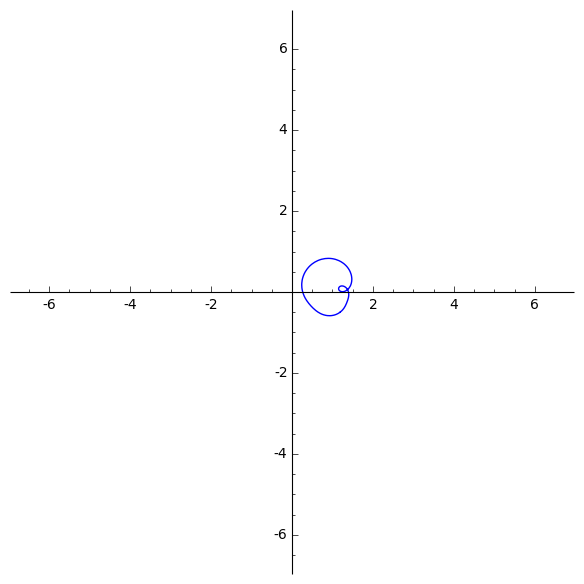
\includegraphics[scale=0.3]{figures/polynome1}\quad
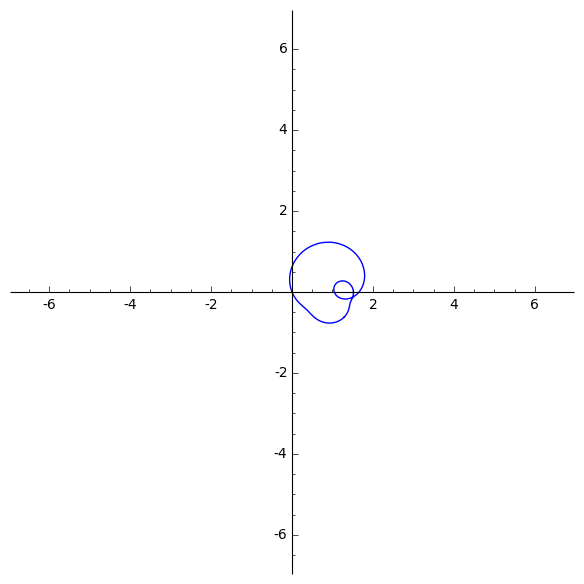
\includegraphics[scale=0.3]{figures/polynome2}\quad
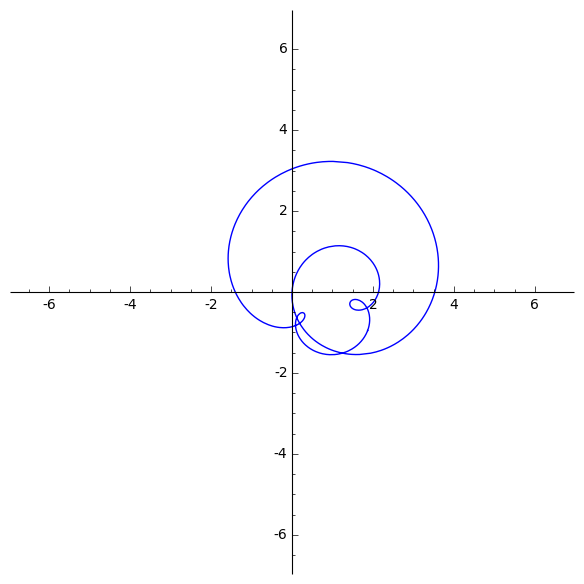
\includegraphics[scale=0.3]{figures/polynome3}
\end{center}
\begin{center}
  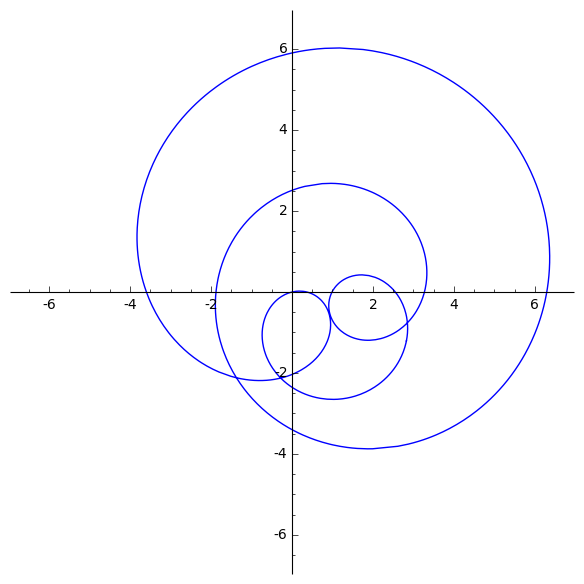
\includegraphics[scale=0.3]{figures/polynome4}\quad
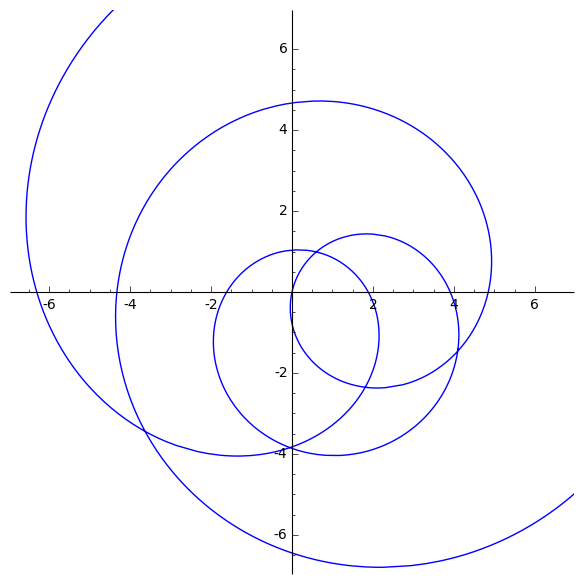
\includegraphics[scale=0.3]{figures/polynome5}\quad
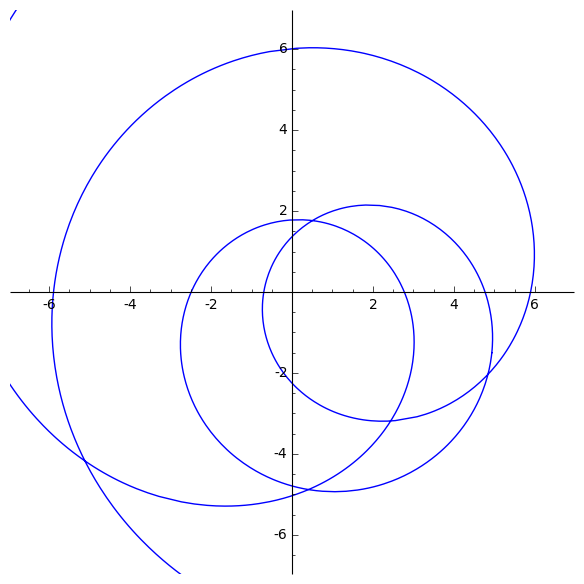
\includegraphics[scale=0.3]{figures/polynome6}
\end{center}

Quand la courbe $\mathcal{C}_r$ passe-t-elle par l'origine ? La courbe passe par l'origine
s'il existe un nombre complexe $re^{\ii t}$ tel que $P(re^{\ii t}) = 0$, c'est-à-dire lorsque 
$P$ admet une racine de module $r$. %D'après le théorème de d'Alembert-Gauss 
On sait qu'un polynôme de degré $n$ a au plus $n$ racines. 
%Alors
Donc il y a au plus $n$ valeurs $r_1,\ldots,r_n$ pour lesquelles 
$\mathcal{C}_{r_i}$ passe par l'origine.
Pour notre exemple de degré $4$, il y a $4$ racines, qui conduisent ici à $4$ modules distincts,
$r_1,\ldots,r_4$.

\medskip

Voici comment procéder :
\begin{itemize}
  \item On commence par définir l'anneau $\Cc[X]$ par \codeinline{R.<X> = CC[]}.
  Les calculs seront donc des calculs approchés avec des nombres complexes.
  Notre polynôme $P$ est défini par \codeinline{P = X^4-X^3+X^2-I*X+1}.
  
  \item 
  Le cercle de rayon $r$ est l'ensemble des complexes de la forme $re^{\ii t}$ pour $t\in [0,2\pi]$.
  La courbe $\mathcal{C}_r$ cherchée est donc l'ensemble 
  $$\mathcal{C}_r = \big\{ P(re^{\ii t}) \mid t \in  [0,2\pi] \big\}.$$
  
  Voici la fonction qui renvoie ce tracé :
\insertcode{algos/intro-polynome-tex2.sage}{intro-polynome.sage (2)}   
  
  \item Une animation est une juxtaposition d'images. 
  On la définit, en visualisant à chaque fois le pavé $[-3,3]\times[-3,3]$, par :
  \begin{lstlisting}
    A = animate( [plot_image_cercle(P,r) for r in srange(0.5,1.5,0.05)],
                 xmin=-3,xmax=3,ymin=-3,ymax=3 )
\end{lstlisting}
%  \centerline{\codeinline{A = animate( [plot_image_cercle(P,r) for r in srange(0.5,1.5,0.05)] )}}  
  puis on l'affiche par \codeinline{A.show()}.
\end{itemize}

\begin{remarque*}
Par défaut \Sage\ fait les calculs dans un ensemble appelé \codeinline{SR} (\emph{Symbolic Ring}).
Dans cet ensemble vous pouvez définir des expressions polynomiales et en trouver les racines.
L'accès aux fonctions spécifiques aux polynômes (comme le degré, les coefficients...) est un peu différent. 
Voici comment déclarer un polynôme, récupérer son degré ainsi que le coefficient devant $X^2$ :
 \insertcode{algos/intro-polynome-tex3.sage}{intro-polynome.sage (3)} 
\end{remarque*}


%--------------------------------------------------------
\subsection{Algorithme de Horner}

L'algorithme de Horner permet d'évaluer rapidement un polynôme $P$ en une valeur $\alpha$.
Voyons comment il fonctionne à la main avec l'exemple de $P(X) = X^5 + X^4 - 5X^3 - 3X - 2$
et $\alpha = 2$.

Sur la première ligne du tableau, on écrit les coefficients de $P$, $a_n,a_{n-1},\ldots,a_1,a_0$.
On reporte en troisième ligne première colonne, $a_n$, le coefficient dominant de $P$.
On multiplie ce nombre par $\alpha$, on l'écrit en deuxième ligne, deuxième colonne, 
% (sur la deuxième ligne, décalé d'un cran à droite),
puis on ajoute $a_{n-1}$ que l'on écrit en troisième ligne, deuxième colonne.
% (sur la troisième ligne juste en dessous). 
Et on recommence. À chaque étape, on multiplie le dernier nombre obtenu par $\alpha$ et on lui ajoute un coefficient de $P$. 
Le dernier nombre obtenu est $P(\alpha)$.

\myfigure{1}{
\tikzinput{fig_formel_polynome01}
}

Ici le dernier nombre est $0$, donc $P(2)=0$. Conclusion : $2$ est racine de $P$.


Avec le même polynôme et $\alpha=-1$ le tableau se complète ainsi :
\myfigure{1}{
\tikzinput{fig_formel_polynome02}
}

ce qui donne $P(-1)=6$.

Ce qui suit formalise cette procédure et montre que l'algorithme de Horner permet des calculs efficaces avec les polynômes.

\begin{tp}
On fixe un corps $K$ et $\alpha\in K$. Soit $P(X) = a_nX^n+a_{n-1}X^{n-1}+\cdots +a_kX^k+\cdots+ a_1X+a_0 \in K[X]$.
%Fixons $\alpha \in K$. 

%Faire les applications avec 
On pourra prendre pour les applications 
$P(X) = X^5 + X^4 - 5X^3 - 3X - 2$ et $\alpha = 2$, puis $\alpha = -1$.

\begin{enumerate}
  \item Compter et comparer le nombre de multiplications nécessaires dans $K$ pour calculer 
  $P(\alpha)$, par :
  \begin{enumerate}
    \item le calcul direct :
    $$P(\alpha) = a_n \alpha^n+a_{n-1} \alpha^{n-1}+\cdots +a_k \alpha^k+\cdots+ a_1 \alpha +a_0,$$
    
    \item l'algorithme de Horner :
    $$P(\alpha) =  \Big(\big((a_n \alpha+a_{n-1})\alpha +a_{n-2} \big) \alpha + \cdots +a_1\Big) \alpha +a_0.$$
    
    \item \'Ecrire une fonction qui calcule $P(\alpha)$ par l'algorithme de Horner.
  \end{enumerate}
  
  \item On formalise le calcul précédent en définissant la suite :
  $$b_{n} = a_n \qquad \text{ puis pour } \qquad n-1\ge k \ge 0\  : \ b_{k} = \alpha b_{k+1}  + a_k.$$
  
  \begin{enumerate}
     
    \item Montrer que dans la division euclidienne de $P(X)$ par $X-\alpha$ qui s'écrit :
    $$P(X) = (X-\alpha) Q(X) + P(\alpha) $$
    le reste $P(\alpha)$ est égal à $b_0$ et le quotient $Q(X)$ est égal au polynôme 
    $b_{n}X^{n-1}+\cdots +b_2X+b_1$ 
    %est constitué des 
    dont les coefficients sont les $b_k$ pour $k\geq 1$.
    
    \emph{Indications.} Pour ce faire développer $(X-\alpha)Q(X)$ et retrouver 
    pour les coefficients de $Q$ la même relation de récurrence que celle 
    définissant la suite des $b_k$.

  
   \item Modifier votre fonction afin qu'elle calcule la suite $(b_{n},b_{n-1},\ldots,b_1,b_0)$
   et qu'elle renvoie le quotient $Q$ et le reste $b_0 = P(\alpha)$.
  
  \item \'Ecrire une fonction qui calcule l'expression d'un polynôme $P(X)$ dans la base
  des $(X-\alpha)^k$, c'est-à-dire calculer les $c_k \in K$ tels que :
  $$P(X) = c_n (X-\alpha)^n+ c_{n-1}(X-\alpha)^{n-1}+ \cdots + c_1(X-\alpha) + c_0.$$
  \end{enumerate}
\end{enumerate}

\end{tp}




\begin{enumerate}
  \item 
  \begin{enumerate}
    \item Le calcul d'un monôme $a_k\cdot \alpha^k$ de degré $k$ nécessite $k$ multiplications, donc pour calculer
    $P(\alpha)$ il faut $n+(n-1)+\cdots+k+\cdots+1+0 = \frac{n(n+1)}{2}$ multiplications (et $n$ additions).
    
    \item La méthode de Horner 
    $$P(\alpha) =  \Big(\big((a_n \alpha+a_{n-1})\alpha +a_{n-2} \big) \alpha + \cdots + a_1\Big) \alpha +a_0.$$
    nécessite seulement $n$ multiplications (et $n$ additions). 
    On passe d'un coût d'ordre $\frac12n^2$ à un coût d'ordre $n$ ; le gain est donc énorme.
     
    \item Pour l'implémentation, on note que la formule de récurrence 
    se fait pour des indices $k$ allant en décroissant.
  
    \insertcode{algos/horner-tex1.sage}{horner.sage (1)}   
  


  \end{enumerate} 
  \item 
  \begin{enumerate}
    \item On note la division euclidienne de $P(X)$ par $X-\alpha$ sous la forme
    $P(X) = (X-\alpha)Q(X) + R$. Le polynôme $Q$ est de degré $n-1$ et on le note
    $Q(X) = b_{n}'X^{n-1}+\cdots+ b_k'X^{k-1}+\cdots +b_2'X+b_1'$ (on veut montrer $b'_k=b_k$).
    Le reste $R$ est de degré strictement inférieur à $\deg (X-\alpha) = 1$ donc $R$ est un polynôme constant.
    En évaluant l'égalité de la division euclidienne en $\alpha$, on a immédiatement $P(\alpha)=R$, 
    que l'on note pour l'instant $b_0'$.
    
    L'égalité $P(X) = (X-\alpha)Q(X) + R$ s'écrit :
    $$P(X) = (X-\alpha)\big(b_{n}'X^{n-1}+\cdots +b_k'X^{k-1}+\cdots +b_2'X+b_1'\big) + b_0'.$$
   On développe le terme de droite et on regroupe les monômes de même degré :
   $$P(X) = b'_{n}X^{n}+(b'_{n-1}-\alpha b_n')X^{n-1} + \cdots + (b'_{k}-\alpha b'_{k+1})X^{k} 
    +\cdots+(b_1'-\alpha b_2')X+(b_0'-\alpha b_1')$$
   On identifie coefficient par coefficient :
   $$\left\{
   \begin{array}{rcl}
   b_n' &=& a_n \\
   b'_{n-1}-\alpha b_n' &=& a_{n-1} \\
   &\cdots& \\
   b'_{k}-\alpha b'_{k+1}&=& a_k \\
   &\cdots& \\
   b_0'-\alpha b_1' &=& a_0 \\
   \end{array}
   \right.
   \qquad \text{ donc }\qquad
 \left\{
   \begin{array}{rcl}
   b_n' &=& a_n \\
   b_{n-1'} &=& \alpha b_n' + a_{n-1} \\
   &\cdots& \\
   b_{k}' &=& \alpha b'_{k+1} + a_k \\
   &\cdots& \\
   b_0'&=& \alpha b_1' + a_0 \\
   \end{array}
   \right.$$
   Les suites $(b_k')$ et $(b_k)$ sont définies par le même terme initial $a_n$ et 
   la même relation de récurrence, elles sont donc égales.
          
    \item On modifie légèrement le code précédent. La suite
    $(b_{n},b_{n-1},\ldots,b_1)$ donne les coefficients de $Q$ (attention au décalage) et $b_0$
    donne le reste qui n'est autre que $P(\alpha)$.
    
    \insertcode{algos/horner-tex2.sage}{horner.sage (2)}   

    \begin{itemize}
      \item Pour notre polynôme $P(X) = X^5 + X^4 - 5X^3 - 3X - 2$ 
    et $\alpha = 2$, l'appel de la fonction définie ci-dessus : \codeinline{division_horner(P,alpha)}
    renvoie un reste $R$ nul et un quotient $Q(X) = X^4 + 3X^3 + X^2 + 2X + 1$.
    Ce qui signifie que $X-2$ divise $P(X)$ ou encore que $P(2)=0$.

      \item Pour ce même polynôme et $\alpha = -1$, la commande 
      \codeinline{division_horner(P,alpha)}
    renvoie $Q(X) =X^4 - 5X^2 + 5X - 8$ et un reste $R = 6$.
    
    \end{itemize}    
    
    \item On obtient les $c_k$ comme restes de divisions euclidiennes successives par $X-\alpha$.
    On commence par la division euclidienne de $P(X)$ par $X-\alpha$.
    On a vu comment calculer le quotient $Q_1$ et le reste $b_0 = P(\alpha)$.
    En évaluant l'expression 
    $P(X) = c_n (X-\alpha)^n+ \cdots + c_1(X-\alpha) + c_0$ en $\alpha$, on voit que l'on a aussi 
    $c_0 = P(\alpha)$ donc $c_0$ est le reste de la première division par $X-\alpha$.
    
    On a donc $P(X) = (X-\alpha)Q_1(X) + c_0$.
    On recommence en divisant $Q_1$ par $X-\alpha$, on obtient un quotient $Q_2$ et un reste qui va être $c_1$. Donc
    $P(X) = (X-\alpha)\big( (X-\alpha)Q_2+c_1 \big) + c_0$.
    
    On continue ainsi de suite jusqu'à ce que le quotient soit nul (au bout de $n+1$ étapes), on a alors 
    $$P(X) =  \Big(\big((c_n (X-\alpha)+c_{n-1})(X-\alpha) +c_{n-2} \big) (X-\alpha) + \cdots c_1\Big) (X-\alpha) +c_0$$    
    soit en développant :
    $$P(X) = c_n (X-\alpha)^n+ \cdots + c_1(X-\alpha) + c_0.$$
    
    Le code suivant renvoie les coefficients $(c_0,c_1,\ldots,c_n)$.
    \insertcode{algos/horner-tex3.sage}{horner.sage (3)} 
    
    \begin{itemize}
      \item Pour $P(X) = X^5 + X^4 - 5X^3 - 3X - 2$ 
    et $\alpha = 2$, la commande \codeinline{developpe_horner(P,alpha)}
    renvoie la liste \codeinline{[0, 49, 74, 43, 11, 1]}, ce qui signifie :
    $$P(X) = 1\cdot(X-2)^5+11\cdot (X-2)^4+43\cdot(X-2)^3+74\cdot(X-2)^2+49\cdot(X-2).$$
    
    
      \item Pour le même polynôme et $\alpha = -1$, la fonction renvoie 
      \codeinline{[6, -17, 11, 1, -4, 1]}, donc
    $$P(X) = 1\cdot(X+1)^5-4\cdot (X+1)^4+1\cdot(X+1)^3+11\cdot(X+1)^2-17\cdot(X+1)+6.$$      
  
    \end{itemize}
  \end{enumerate}
\end{enumerate}


%--------------------------------------------------------
\subsection{Interpolation de Lagrange}




\begin{theoreme}[Interpolation de Lagrange]
Soient $(x_i,y_i)$, $i=0,\ldots,n$, une suite de $n+1$ points, d'abscisses deux à deux distinctes. 
Il existe un unique polynôme $P$ de degré inférieur ou égal à $n$ tel que
$$P(x_i)=y_i \quad \text{ pour } i=0,\ldots,n.$$
\end{theoreme}

En particulier, pour toute fonction $f$ continue sur un intervalle contenant $x_0,\ldots,x_n$, 
il existe un unique polynôme $P$ de degré inférieur ou égal à $n$ tel que
$$P(x_i)=f(x_i) \quad \text{ pour } i=0,\ldots,n.$$


\begin{tp}
\sauteligne
\begin{enumerate}
  \item Montrer l'unicité du polynôme $P$ dans le théorème d'interpolation de Lagrange. 
  
  \item Pour l'existence, étant donnés $x_0,\ldots, x_n$, on définit les polynômes de Lagrange $L_0,L_1,\ldots,L_n$:
  $$L_i(X) = \prod_{j \neq i} \frac{X-x_j}{x_i-x_j}.$$
  Montrer que le polynôme :
  $$P(X) = \sum_{i=0}^{n} y_i L_i(X)$$
  répond au problème : il est de degré inférieur ou égal à $n$ et $P(x_i)=y_i$  pour $i=0,\ldots,n$.
    
  \item \'Ecrire une fonction qui, étant donnée une liste de points, renvoie le polynôme
  d'interpolation $P$.
  
  \item Interpoler la fonction définie par $f(x) = \sin(2\pi x)e^{-x}$
  sur l'intervalle $[0,2]$ pour une subdivision régulière de $n+1$ points.
  Tracer les graphes de la fonction $f$ et des polynômes d'interpolation
  correspondant à différentes valeurs de $n$.
  
  \item Faire le même travail avec la fonction définie par $f(x) = \frac{1}{1+8x^2}$
  sur l'intervalle $[-1,1]$ pour une subdivision régulière de $n+1$ points.
  Quel problème apparaît ? C'est le \emph{phénomène de Runge}.
\end{enumerate}
\end{tp}

\begin{enumerate}
  \item Supposons que $P$ et $Q$ soient deux polynômes de degré inférieur à $n$ vérifiant
  $P(x_i)=y_i$ et $Q(x_i)=y_i$ pour $i=0,\ldots,n$. Alors le polynôme $P-Q$ vérifie
  $(P-Q)(x_i)=0$ pour $i=0,\ldots,n$. Ainsi $P-Q$ est un polynôme de degré inférieur ou égal à $n$ 
  ayant $n+1$ racines. %D'après le théorème de d'Alembert-Gauss, 
  C'est donc nécessairement le polynôme nul.
  Ainsi $P-Q=0$, donc $P=Q$.
  
  \item Les polynômes $L_i$ sont de degré exactement $n$ et sont définis de sorte que
  $$L_i(x_i) = 1 \quad \text{ et } \quad L_i(x_j)=0 \quad\text{ pour } j\neq i.$$
  Il est alors clair que $P(X) = \sum_{j=0}^{n} y_j L_j(X)$
  est aussi de degré inférieur ou égal à $n$ et vérifie pour  $i=0,\ldots,n$ : 
  $$P(x_i)=  \sum_{j=0}^{n} y_j L_j(x_i) = y_iL_i(x_i) = y_i.$$
  
   
  \item On commence par définir :
  \begin{itemize}
    \item \codeinline{R.<X> = RR[]} : l'anneau de polynômes (les coefficients sont des réels approchés) ;
    \item \codeinline{f = sin(2*pi*x)*exp(-x)} : la fonction ;
    \item \codeinline{liste_points = [ (2*i/n, f(x=2*i/n)) for i in range(n+1) ]} : une liste de points
    du graphe de $f$.
  \end{itemize}

  La fonction suivante renvoie le polynôme interpolateur d'une liste de points.
  
   \insertcode{algos/interpolation-tex.sage}{interpolation.sage}   
  
  \item Voici les tracés de la fonction (en rouge) définie par $f(x) = \sin(2\pi x)e^{-x}$ 
    et des polynômes d'interpolation (en bleu) pour $n=3,4,5,6,7$ et $8$.
    Pour $n=4$, le polynôme est le polynôme nul. À partir de $n=8$, il devient difficile de distinguer le
    graphe de la fonction du graphe du polynôme.
  
  \begin{center}
    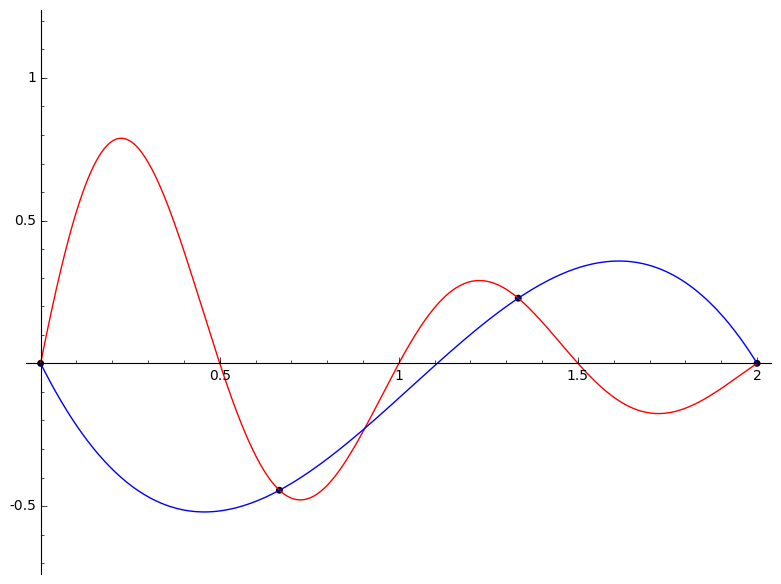
\includegraphics[scale=0.2]{figures/lagrange1}\quad
    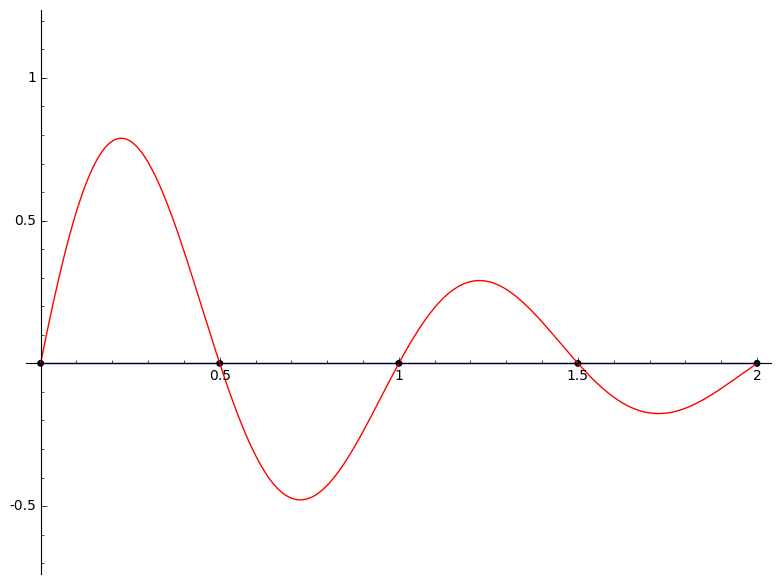
\includegraphics[scale=0.2]{figures/lagrange2}\quad
    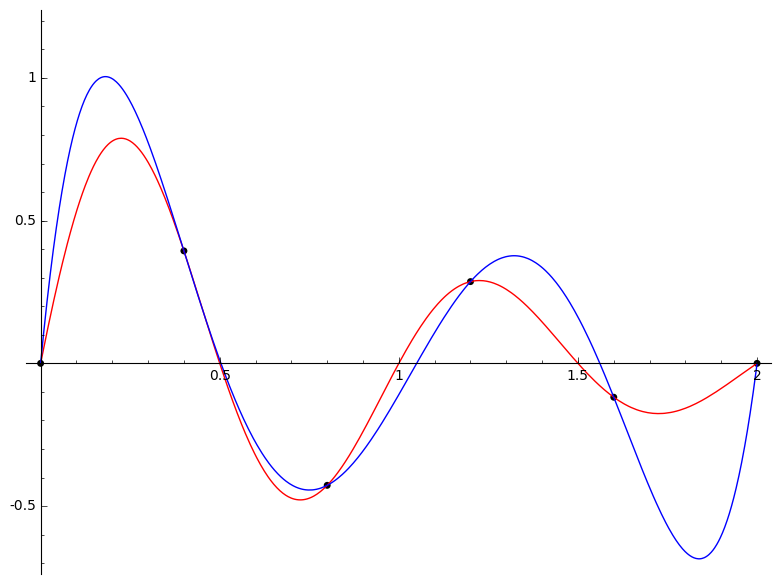
\includegraphics[scale=0.2]{figures/lagrange3}
  \end{center}
  \begin{center}
    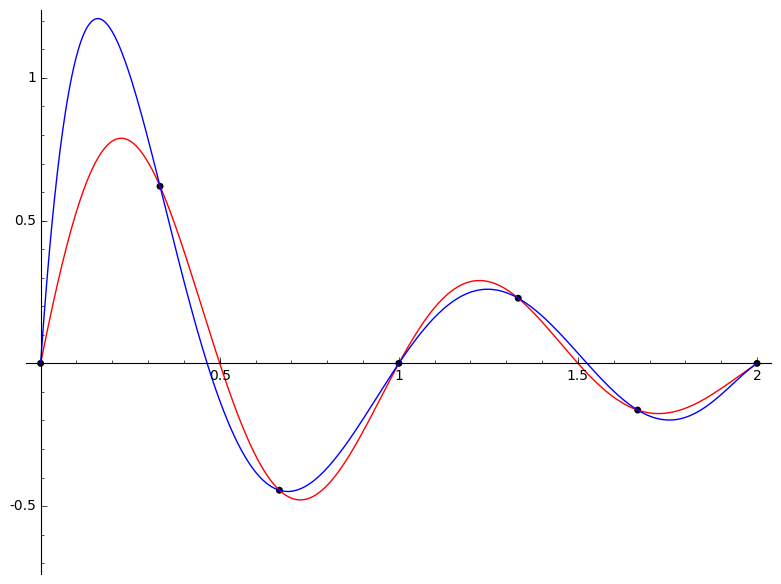
\includegraphics[scale=0.2]{figures/lagrange4}\quad
    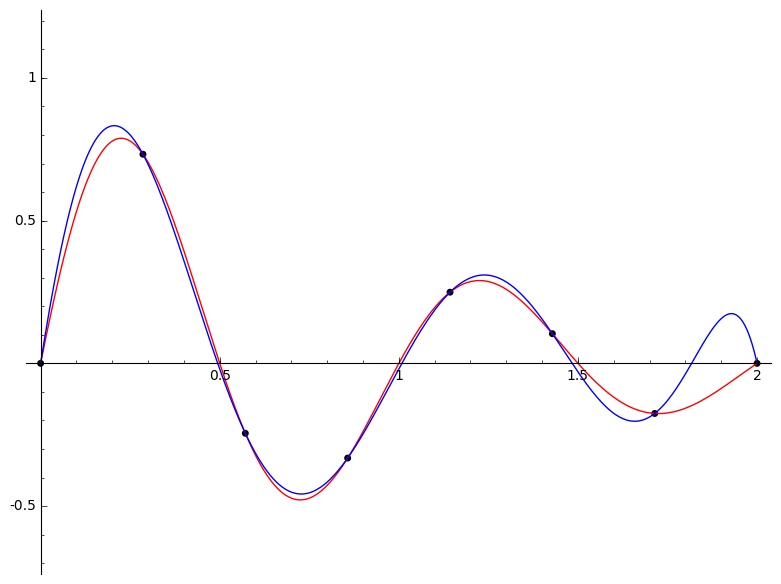
\includegraphics[scale=0.2]{figures/lagrange5}\quad
    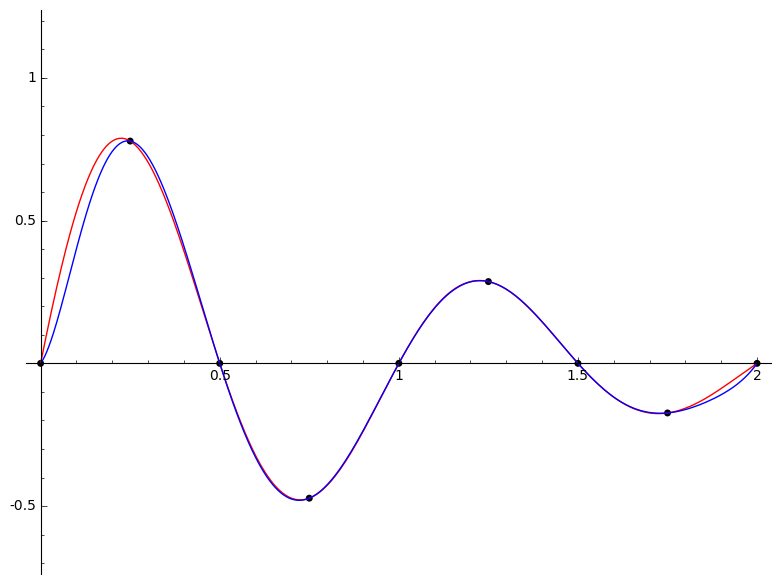
\includegraphics[scale=0.2]{figures/lagrange6}
  \end{center}
  
  \item Voici l'interpolation de $f(x) = \frac{1}{1+8x^2}$
  pour $n=7,10$ et $18$. La zone centrale de la courbe est bien interpolée mais, autour de $-1$ et $+1$,
  des <<bosses>>\ apparaissent. Ces bosses deviennent de plus en plus grandes en se décalant vers les extrémités. 
  Il y a convergence simple mais pas convergence uniforme. Pour éviter ce phénomène, il faudrait mieux choisir les 
  $x_i$.
  \begin{center}
    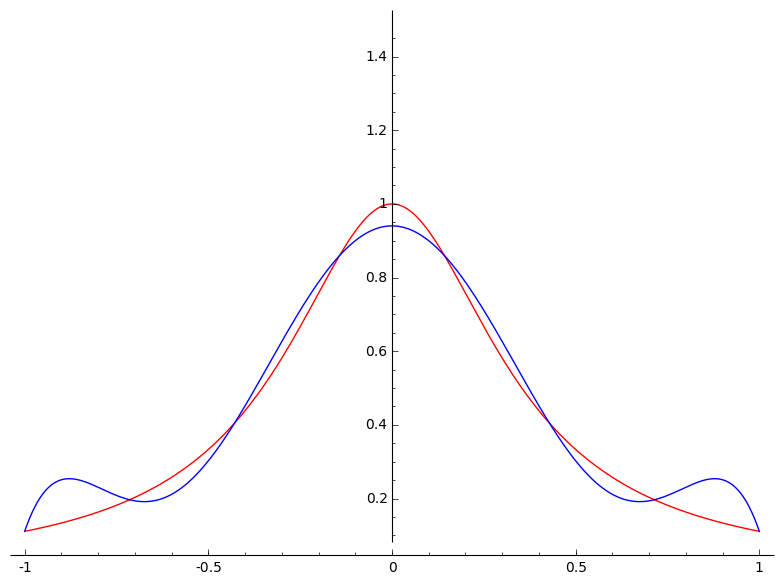
\includegraphics[scale=0.22]{figures/runge1}\quad
    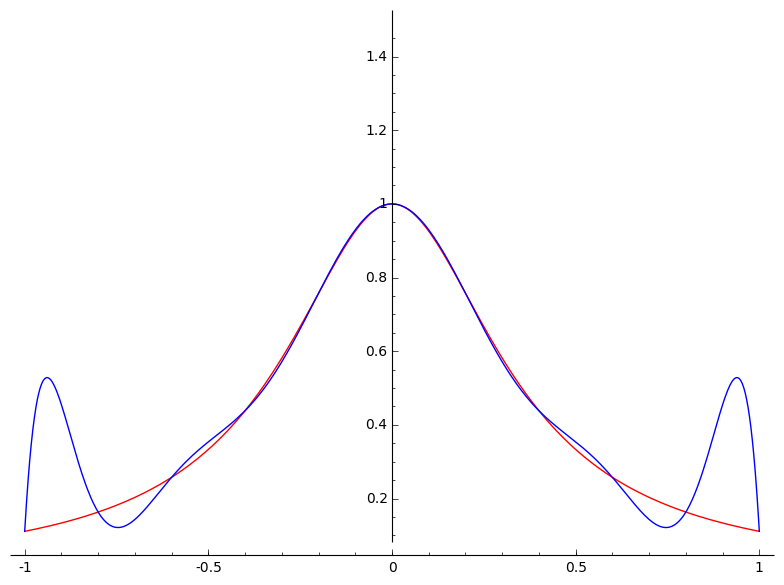
\includegraphics[scale=0.22]{figures/runge2}\quad
    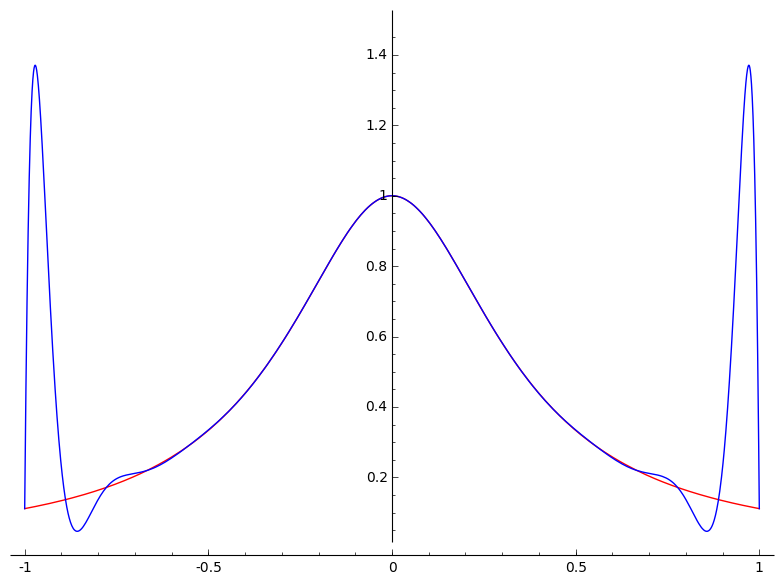
\includegraphics[scale=0.22]{figures/runge3}
  \end{center} 
  
\end{enumerate}

\finchapitre

\end{document}

